\chapter{Herramientas y metodologías}
\label{chap:herramientas_y_metodologias}

    Construir una arquitectura distribuida de forma individual exige combinar rigor en el código con agilidad en las entregas. Se adoptó una metodología ágil adaptada, reforzada con la práctica de desarrollo guiado por pruebas o TDD (\emph{Test-Driven Development}). Esta disciplina permitió dividir el desarrollo en ciclos cortos de especificación, codificación y verificación inmediata. Cada módulo quedaba validado antes de enlazarlo con el resto del sistema.

    TDD blindó las partes más sensibles del dominio: el cálculo de saldos en gastos compartidos y la concurrencia en la reserva de habitaciones. Redactar las pruebas con anterioridad fijó el comportamiento esperado de servicios y repositorios sin ambigüedades. Durante este proceso, se emplearon modelos de lenguaje como asistentes de apoyo para explorar casos límite en las aserciones y sugerir refactorizaciones orientadas a principios SOLID (\emph{Single responsibility, Open-closed, Liskov substitution, Interface segregation, Dependency inversion}).

    El stack técnico se seleccionó priorizando tipado estático, rendimiento transaccional y bajo acoplamiento:

\begin{itemize}
\item \textbf{Entorno de desarrollo}: Antigravity centralizó el espacio de trabajo coordinando la edición simultánea del backend y los microservicios, terminales concurrentes y automatización de tareas.
\item \textbf{Lógica de negocio y servicios}: el backend principal se programó en Java 21 sobre Spring Boot 3, integrando Spring AI para la comunicación con LLMs y la ejecución de llamadas a herramientas. Paralelamente, se construyó un servidor MCP (\emph{Model Context Protocol}) en Node.js y TypeScript que expone sus endpoints mediante \emph{Server-Sent Events} (SSE).
\item \textbf{Interfaz web y empaquetado móvil}: el cliente web se programó en React con TypeScript y empaquetado con Vite. Tailwind CSS resolvió el diseño visual y TanStack Query gestionó las consultas en segundo plano. Mediante Capacitor se generó el paquete nativo instalable en Android reutilizando el código web.
\item \textbf{Almacenamiento de datos}: PostgreSQL administra las transacciones relacionales, consumidas desde Java mediante JPA e Hibernate con bloqueos explícitos para evitar conflictos de concurrencia.
\item \textbf{Prototipado y diagramación}: las pantallas se diseñaron en Figma para escritorio y móvil. PlantUML generó los diagramas UML directamente desde ficheros de texto plano, mientras draw.io sirvió para los esquemas arquitectónicos.
\item \textbf{Control de versiones y cronograma}: GitHub alojó los repositorios bajo un flujo estricto de ramas y solicitudes de extracción (\emph{pull requests}). El seguimiento de tiempos y fechas límite se controló en GanttProject.
\end{itemize}

    Los siguientes apartados profundizan en la disciplina metodológica elegida y en la función de cada herramienta dentro de la arquitectura del proyecto.

\section{Metodologías usadas}
\label{Metodologias usadas}

    La guía SWEBOK (\emph{Software Engineering Body of Knowledge}) \cite{SWEBOK2014} divide la ingeniería del software en procesos disciplinados para planificar, ejecutar y controlar el desarrollo frente a restricciones reales. Elegir un método de trabajo determina cómo evoluciona el código y cómo se responde a cambios en los requisitos sin comprometer la estabilidad del sistema.

\subsection{Revisión de enfoques metodológicos}

    El modelo tradicional en cascada exige completar y congelar cada fase antes de iniciar la siguiente: requisitos, diseño, codificación, verificación y entrega. Si bien funciona en proyectos con especificaciones cerradas y contratos rígidos, fracasa al integrar servicios desacoplados o protocolos emergentes como MCP. Descubrir un fallo de integración en la fase final de pruebas dispararía el coste de rehacer módulos enteros.

    Scrum estructura el trabajo en iteraciones cortas llamadas \emph{sprints}, orientadas a entregar incrementos funcionales cada dos o cuatro semanas. Reparte responsabilidades entre perfiles definidos (\emph{Scrum Master}, \emph{Product Owner}, equipo de desarrollo) y exige reuniones periódicas de sincronización y retrospectiva. Pese a dominar en la industria corporativa, su burocracia de reuniones pierde sentido en un proyecto individual sin equipo que coordinar. La figura \ref{fig:agile_vs_waterfall} refleja la comparativa histórica de tasas de éxito entre ambos enfoques.

\begin{figure}[H]
    \centering
    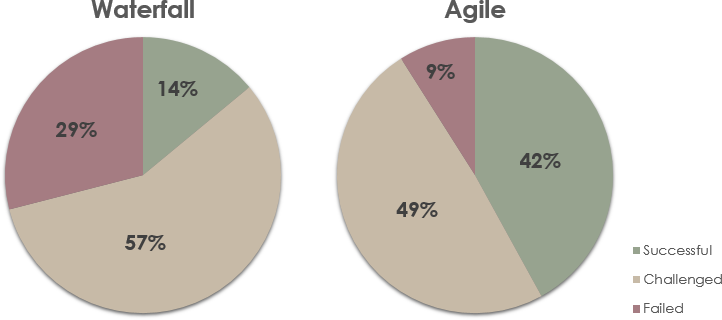
\includegraphics[width=0.68\textwidth]{HerramientasYMetodologias/img/Waterfall_vs_agile.png}
    \caption{Diferencia de éxito entre metodologías ágiles y tradicionales en cascada}
    \label{fig:agile_vs_waterfall}
\end{figure}

    Kanban elimina las cadencias temporales fijas y se centra en limitar el trabajo en curso o WIP (\emph{Work In Progress}). Las tareas avanzan a través de columnas de estado en un tablero visual (figura \ref{fig:tablero_kanban}): pendientes, en desarrollo y completadas. Este flujo continuo permite priorizar el trabajo según cuellos de botella reales, facilitando al programador concentrarse en un solo componente hasta cerrarlo.

\begin{figure}[H]
    \centering
    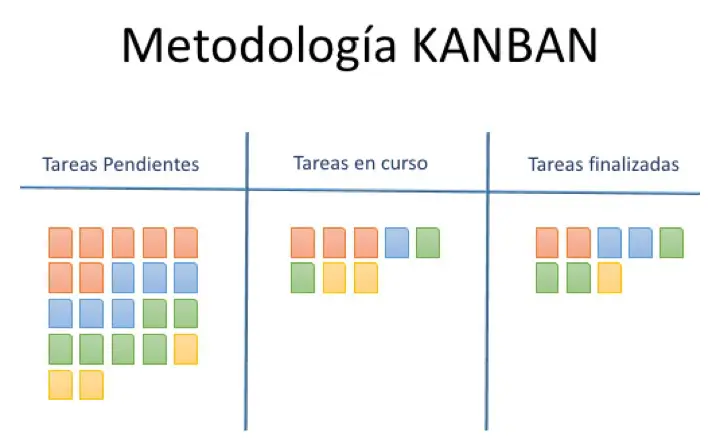
\includegraphics[width=0.68\textwidth]{HerramientasYMetodologias/img/Kanban.png}
    \caption{Tablero Kanban representativo del flujo de desarrollo ágil}
    \label{fig:tablero_kanban}
\end{figure}

    La programación extrema (\emph{Extreme Programming} o XP) antepone la excelencia en el código a la gestión burocrática. Sus pilares incluyen la refactorización continua, la integración frecuente y el desarrollo guiado por pruebas o TDD (\emph{Test-Driven Development}). En TDD, los tests se redactan antes que el código de producción, garantizando que cada función responda a una necesidad validada y medible.

\subsection{Análisis comparativo y selección para el proyecto}

    La arquitectura de Colivi —un backend modular en Spring Boot 3, un servidor MCP independiente en Node.js, un cliente web en React y el paquete móvil con Capacitor— hacía inviable una cascada estricta. Conectar herramientas de inteligencia artificial con inferencia remota exigía experimentar con esquemas JSON y ajustar contratos sobre la marcha.

    Scrum tampoco encajaba en un escenario unipersonal sin ceremonias diarias. Por estas razones, se diseñó una estrategia híbrida adaptada a las necesidades reales del desarrollo:

\begin{itemize}
\item \textbf{Gestión del flujo de trabajo}: Kanban organizó el avance técnico mediante un tablero en GitHub Projects, vinculando incidencias, dependencias y confirmaciones de código sin imponer cortes temporales artificiales.
\item \textbf{Disciplina técnica con TDD}: las prácticas de XP guiaron la implementación mediante el ciclo de diseño, prueba y refactorización resumido en la figura \ref{fig:TDD}. Este mecanismo protegió el cálculo financiero de deudas y la reserva concurrente de habitaciones, forzando un diseño desacoplado bajo principios SOLID (\emph{Single responsibility, Open-closed, Liskov substitution, Interface segregation, Dependency inversion}).
\item \textbf{Integración asistida}: el entorno Antigravity aceleró la formulación de baterías de pruebas con JUnit y Mockito, complementando la inspección manual con compilaciones automatizadas en ramas de características (\emph{feature branches}).
\end{itemize}

\begin{figure}[H]
    \centering
    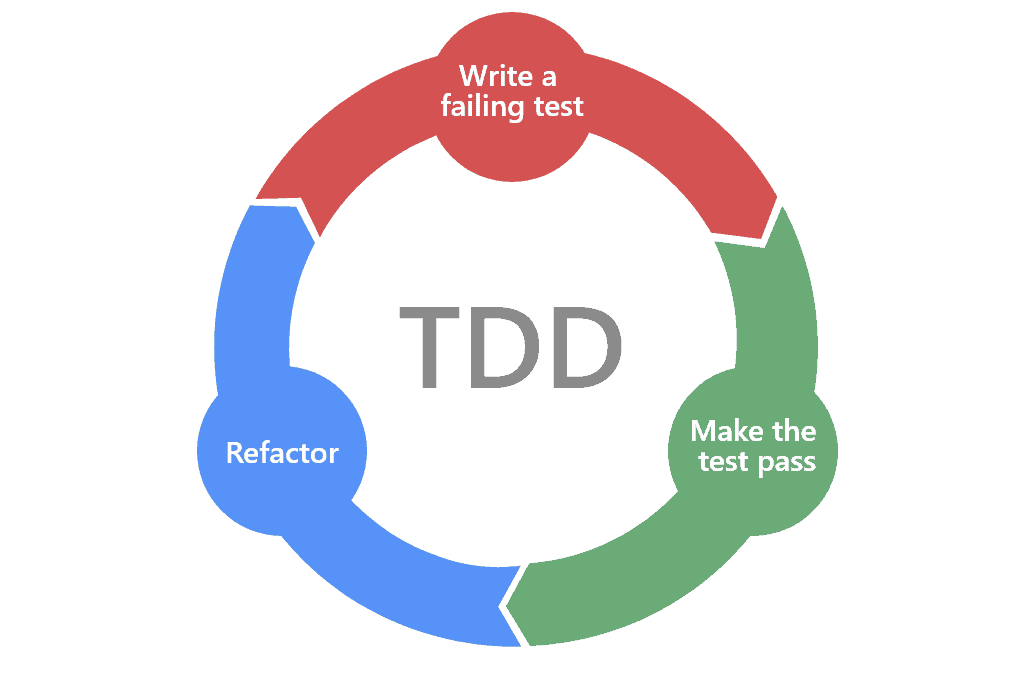
\includegraphics[width=0.68\textwidth]{HerramientasYMetodologias/img/TDD.png}
    \caption{Ciclo iterativo de la metodología TDD (\emph{Test-Driven Development})}
    \label{fig:TDD}
\end{figure}

\clearpage

\section{Herramientas usadas}
\label{sec:herramientas_usadas}

    En esta sección se describen los entornos, lenguajes, marcos de trabajo y utilidades auxiliares que se utilizaron a lo largo del ciclo de vida del proyecto, justificando técnicamente la elección de cada componente frente a otras alternativas disponibles.

\subsection{Entornos de desarrollo y asistencia técnica}
\label{subsec:entornos_desarrollo}

    Para la construcción del sistema se seleccionaron entornos de trabajo específicos en función de las demandas de cada capa de la arquitectura (figura~\ref{fig:entornos_desarrollo}). En el caso del backend y la orquestación general de servicios, se utilizó Antigravity como entorno de trabajo integrado. Esta herramienta proporcionó una gestión eficiente de los espacios de trabajo sobre los repositorios del proyecto, combinando terminales concurrentes, ejecución de contenedores locales y soporte nativo para flujos de codificación asistida. Frente a entornos tradicionales como Eclipse o NetBeans, Antigravity ofreció un consumo de recursos sensiblemente menor y una navegación ágil entre el código del servidor en Spring Boot y el microservicio auxiliar en Node.js.

    Para el desarrollo del frontend web y la capa móvil se optó por Visual Studio Code. Su ecosistema de extensiones, especialmente las relativas al análisis estático de TypeScript, el formateo con Prettier y la integración de ramas con Git, permitió mantener un ritmo de desarrollo uniforme. Aunque se evaluó la posibilidad de unificar todo el trabajo bajo un único entorno pesado como IntelliJ IDEA Ultimate, se prefirió la combinación de Antigravity y Visual Studio Code por su ligereza y facilidad de adaptación al cambio constante de contexto entre lenguajes.

    Por último, en lo relativo al soporte móvil, se recurrió a Android Studio de manera puntual. Al basarse la vertiente móvil en una aproximación híbrida mediante Capacitor, el grueso de la lógica se implementó en la base web; no obstante, Android Studio resultó indispensable para compilar el código nativo, generar la clave de firmado del paquete de aplicación Android o APK (\emph{Android Package Kit}), depurar fallos en el puente de comunicación mediante el inspector web de Android y realizar pruebas sobre emuladores oficiales con distintas versiones del sistema operativo.

\begin{figure}[H]
	\centering
	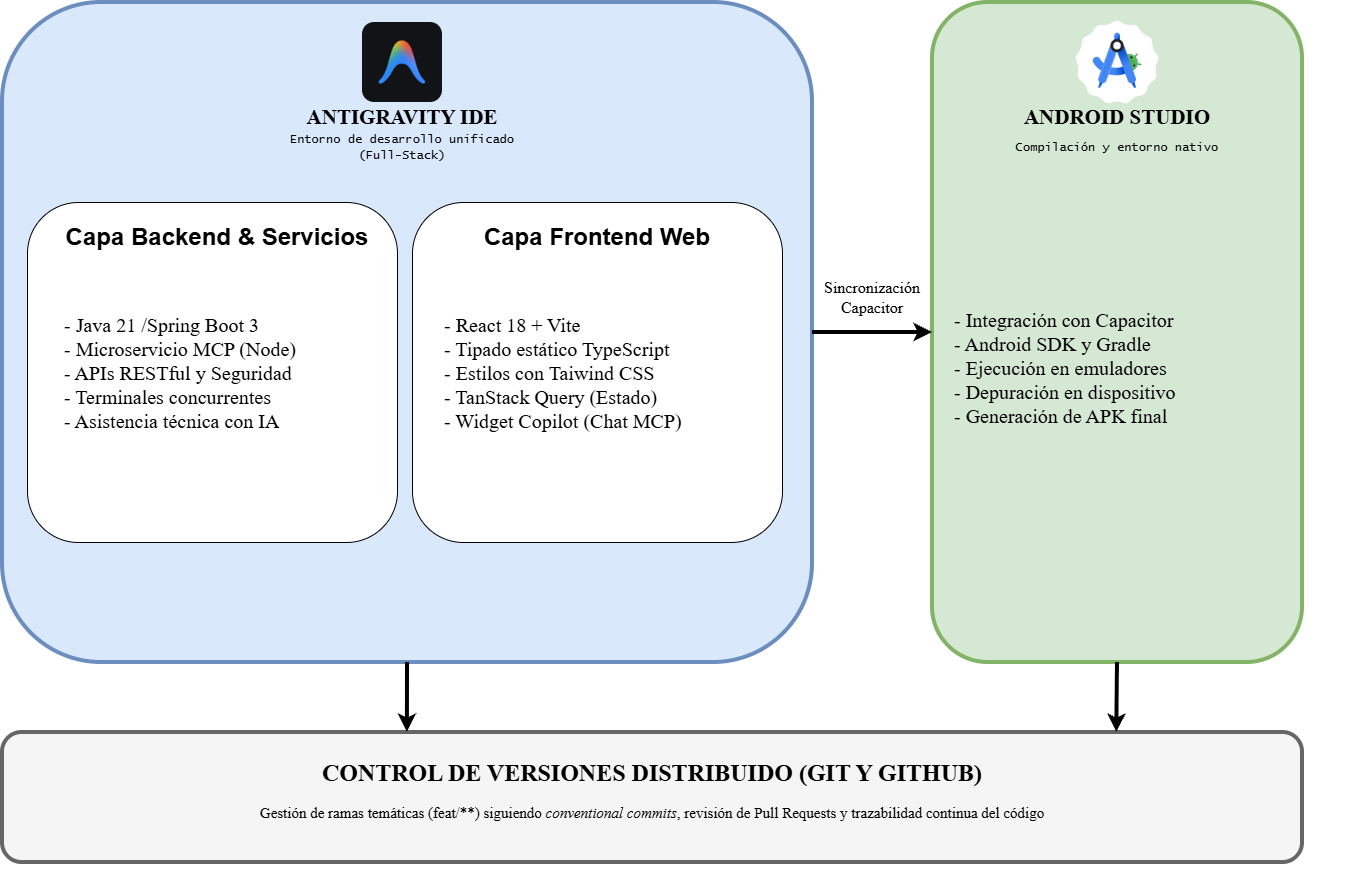
\includegraphics[width=0.68\textwidth]{HerramientasYMetodologias/img/entornos_desarrollo.png}
	\caption{Entornos de desarrollo utilizados en el proyecto. Elaboración propia}
	\label{fig:entornos_desarrollo}
\end{figure}

\subsection{Lenguajes, marcos de trabajo y servicios}
\label{subsec:lenguajes_marcos_servicios}

    La arquitectura distribuida de Colivi requirió una selección tecnológica coherente entre sus diferentes módulos operativos. Para el backend se eligió Java 21 junto con el marco de trabajo Spring Boot 3. La versión 21 de Java aportó características de lenguaje consolidadas como los registros (\emph{records}) y la concordancia de patrones (\emph{pattern matching}), lo que redujo de forma sustancial la redundancia en los objetos de transferencia de datos o DTO (\emph{Data Transfer Object}). Por su parte, Spring Boot 3 ofreció una base robusta para la gestión de inyección de dependencias, transacciones relacionales y seguridad perimetral sin estado mediante Spring Security y filtros de autenticación basados en tókenes web de JSON o JWT (\emph{JSON Web Tokens}). Frente a alternativas como Django en Python o Express en Node.js, Spring Boot garantizó un tipado estricto en la lógica de negocio contable y facilitó la integración directa con Spring AI para interactuar con modelos de lenguaje remotos a través de la interfaz de programación de aplicaciones o API (\emph{Application Programming Interface}) de Groq. En el microservicio del asistente inteligente se optó por Node.js con TypeScript, implementando la especificación del protocolo de contexto de modelo o MCP (\emph{Model Context Protocol}). Se decidió desacoplar este módulo del backend principal para permitir que el servidor de herramientas operara de manera independiente, comunicándose mediante transporte por eventos enviados por el servidor o SSE (\emph{Server-Sent Events}). TypeScript proporcionó la comprobación estática de tipos necesaria para garantizar que los esquemas de entrada y salida de las herramientas del asistente concordaran con los contratos esperados por el orquestador.

    En el desarrollo de la interfaz web se seleccionó React en su versión 18 sobre la herramienta de empaquetado Vite, escribiendo el código íntegramente en TypeScript. A diferencia de JavaScript plano, el uso de TypeScript evitó inconsistencias comunes en tiempo de ejecución al interactuar con las respuestas del servidor. Vite se prefirió frente a Create React App debido a su velocidad de compilación mediante módulos de ECMAScript (\emph{ES Modules}) y al reemplazo en caliente de módulos o HMR (\emph{Hot Module Replacement}). Para el diseño visual se adoptó Tailwind CSS, aprovechando su enfoque de utilidades para estructurar interfaces adaptables sin abandonar los archivos de componentes. La sincronización del estado del servidor se gestionó con TanStack Query, resolviendo de manera transparente el almacenamiento en caché, la invalidación de consultas y la actualización en segundo plano de datos dinámicos como los balances de gastos o las alertas del hogar. Para la aplicación móvil se utilizó Capacitor como puente de integración sobre la base de React. En lugar de desarrollar una aplicación móvil desde cero en Kotlin o emplear marcos de trabajo separados como React Native, Capacitor permitió reutilizar más del 90\% del código del cliente web, envolviendo la interfaz en una vista web nativa con acceso directo a las características del dispositivo. Esta decisión optimizó el tiempo de desarrollo, asegurando una experiencia idéntica entre la versión de navegador y la aplicación instalada en el teléfono.

\subsection{Almacenamiento y persistencia de datos}
\label{subsec:almacenamiento_persistencia}

    La persistencia del sistema se sustentó en el sistema gestor de bases de datos relacionales PostgreSQL en su versión 16 (figura~\ref{fig:postgresql_logo}). La naturaleza transaccional de Colivi —donde coexisten balances contables de facturas, reservas de habitaciones con control de solapamiento de fechas y auditorías de actividad— exigía el cumplimiento íntegro de las propiedades de atomicidad, consistencia, aislamiento y durabilidad o ACID (\emph{Atomicity, Consistency, Isolation, Durability}). PostgreSQL demostró un comportamiento idóneo en el manejo de restricciones de integridad referencial complejas y consultas analíticas frente a motores no relacionales como MongoDB, los cuales se descartaron por carecer de mecanismos nativos estrictos para la resolución de saldos monetarios compartidos. La interacción entre la base de datos y la capa de dominio en Java se canalizó mediante la especificación JPA y el motor Hibernate, definiendo entidades bien mapeadas y repositorios con consultas específicas para mitigar problemas comunes de rendimiento como el cuello de botella de consultas secundarias sucesivas o problema de $N+1$.

\begin{figure}[H]
	\centering
	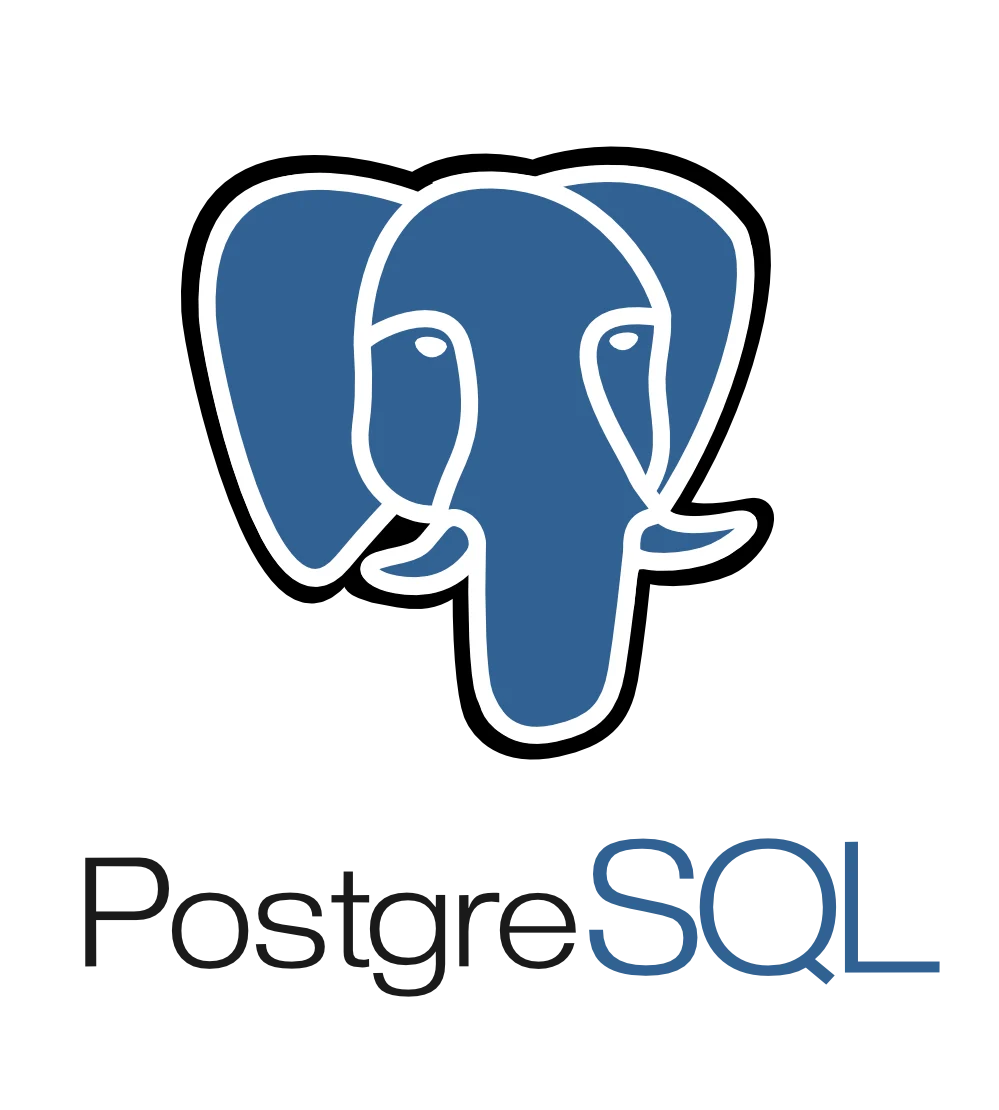
\includegraphics[width=0.45\textwidth]{HerramientasYMetodologias/img/postgresql_logo.png}
	\caption{Sistema gestor de bases de datos PostgreSQL}
	\label{fig:postgresql_logo}
\end{figure}

\subsection{Control de versiones, infraestructura y utilidades auxiliares}
\label{subsec:control_versiones_infraestructura}

    Para la gestión del código fuente se empleó Git como sistema de control de versiones distribuido, alojando los repositorios centrales en la plataforma GitHub. El progreso técnico se organizó siguiendo un flujo de trabajo riguroso basado en ramas y solicitudes de incorporación de cambios o PR (\emph{Pull Requests}). Esta estrategia permitió auditar cada funcionalidad antes de consolidarla en la rama de desarrollo, manteniendo un historial limpio de cambios y vinculando de forma unívoca cada confirmación con las tareas planificadas.

    La contenedorización de los servicios locales se resolvió mediante Docker y Docker Compose. Se definieron archivos de configuración para desplegar simultáneamente la base de datos PostgreSQL, el backend en Spring Boot y el servidor MCP, garantizando que el entorno de ejecución fuera reproducible tanto en equipos de desarrollo como en las fases de despliegue sobre Microsoft Azure.

    Para la fase de diseño visual se utilizó Figma (figura~\ref{subfig:figma}) para maquetar la guía de estilos, los esquemas alámbricos y los prototipos de pantalla en resolución de escritorio y móvil, estableciendo la disposición de las tarjetas de alojamiento y los tableros del hogar antes de iniciar la maquetación.

    Para el modelado formal de la arquitectura y el comportamiento del sistema se empleó PlantUML (figura~\ref{subfig:plantuml}), lo que permitió versionar los diagramas de casos de uso y de secuencia como código fuente dentro del propio repositorio de documentación. Aquellos diagramas de bloques generales de alto nivel se confeccionaron con draw.io por su rapidez para exportar composiciones visuales limpias.

    Finalmente, la verificación de los puntos de acceso de la API y las pruebas de comunicación de eventos SSE se realizaron mediante Postman (figura~\ref{subfig:postman}) y cURL, comprobando manualmente los encabezados de autenticación JWT y los códigos de estado HTTP antes de proceder a la automatización de las baterías de pruebas unitarias e integradas con JUnit 5 y Mockito.

\begin{figure}[H]
	\centering
	\begin{subfigure}[b]{0.32\textwidth}
		\centering
		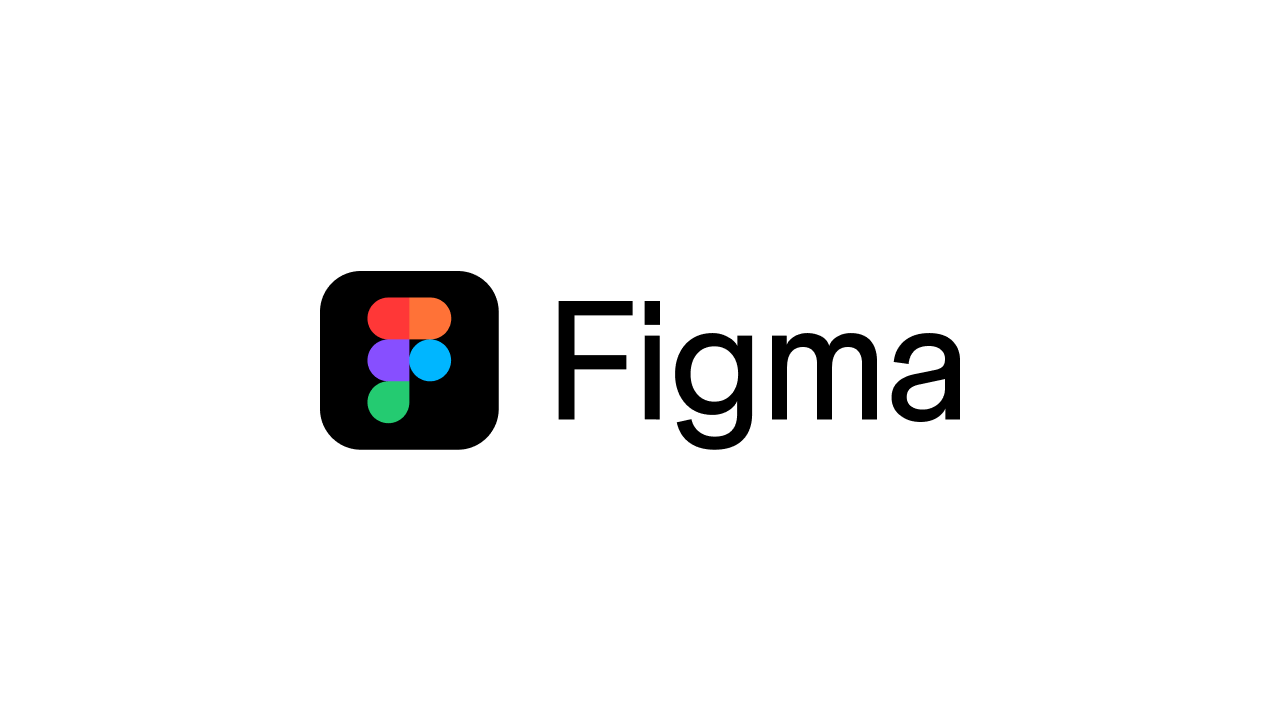
\includegraphics[width=\linewidth,height=2.8cm,keepaspectratio]{HerramientasYMetodologias/img/figma.png}
		\caption{Figma}
		\label{subfig:figma}
	\end{subfigure}
	\hfill
	\begin{subfigure}[b]{0.32\textwidth}
		\centering
		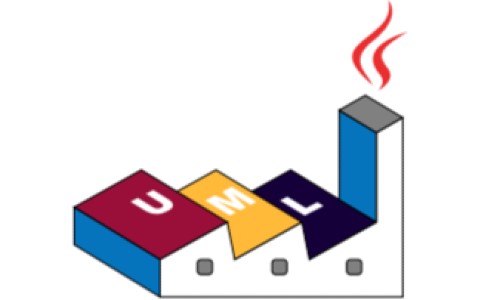
\includegraphics[width=\linewidth,height=2.8cm,keepaspectratio]{HerramientasYMetodologias/img/plantuml.png}
		\caption{PlantUML}
		\label{subfig:plantuml}
	\end{subfigure}
	\hfill
	\begin{subfigure}[b]{0.32\textwidth}
		\centering
		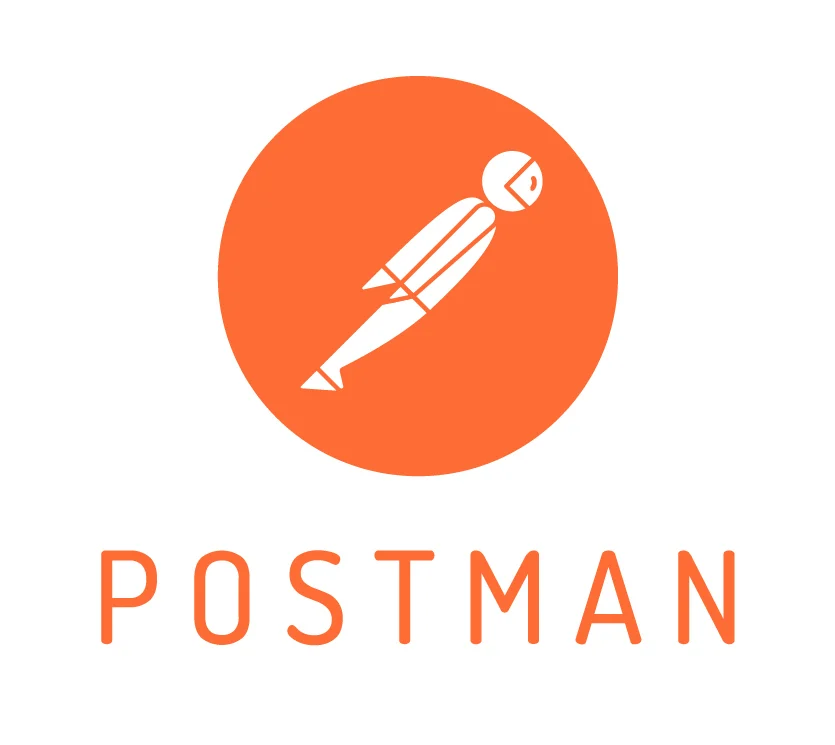
\includegraphics[width=\linewidth,height=2.8cm,keepaspectratio]{HerramientasYMetodologias/img/postman.png}
		\caption{Postman}
		\label{subfig:postman}
	\end{subfigure}
	\caption{Herramientas auxiliares empleadas para diseño de interfaz, modelado y verificación de API}
	\label{fig:herramientas_auxiliares}
\end{figure}